%\linenumbers*
\chapter{EFFECT OF CONTINUOUS AND DISCONTINUOUS STORM ON SOIL EROSION}
\label{sec:EFFECTSOFCONTINOUSANDDISCONTINUSSTORM}

\section{Introduction}
\label{sec:ContinousAndDiscontinousStormIntroduction}

As indicated previously (see page \pageref{sec:ClimateGeneratorCLIGEN}),
effective rainfall duration ($D$, minute), which
is one of four parameters that describe rainfall characteristics in CLIGEN
data, is calculated by discarding no-rain periods within storm duration. Only
rainfall periods within storm duration are aggregated into a ``gapless''
rainfall storm. By removing no-rain periods, actual rainfall duration is
reduced so that average intensity of rainfall storm is increased. Consequently,
the removal of no-rain periods, which is termed as Within-Storm Gaps (WSGs) for
this research, may have effects on erosion modelling.

Therefore, this chapter examines the effect of the removal of WSGs on
runoff and soil loss estimations. Continuous (without WSGs) and discontinuous
(with WSGs) storms are distinguished by the existence of WSGs within the storm
duration. Three process-based models---WEPP, EUROSEM and an additional model,
RillGrow---were used in this chapter. Runoff and soil loss rate were estimated
by these models and the outputs were examined in terms of their relationships to
WSGs.

WEPP and EUROSEM have shown contrasting results in the previous chapter. Thus,
RillGrow was used here with an intention to strengthen the model estimation
results by increasing the number of model predictions. Although the outputs from
three erosion models may still give three very different results---this actually
was the case---employing all three models may also give a stronger argument that
the removal of WSGs does (or does not) have an impact on runoff and soil loss
simulations.
The main aim of this investigation is to find out whether WSGs influence runoff
and soil loss generations. The more important question is, however, how WSGs
influence runoff and soil erosion. This is more difficult to answer even when a
single erosion model is used.

\section{Simulation Data and Methods}
\label{sec:ContinousAndDiscontinousStormMethods}

Event rainfall recorded on 11 October 2000 at Southover station (S) (see Table
\ref{tab:DetailsOfDataStations}) was selected because this event was a
distinctive storm with a large amount of rainfall. The event also includes a
number of WSGs in the total storm duration. The total rainfall amount of the
storm is 89.9 mm. This event is considered to be responsible for the severe
flood incidents in the study region \citep{boardman2001-346}.

Only breakpoint data type, which retains WSGs, was used in this chapter because
CLIGEN data remove WSGs by its design specification. Also, temporal resolution of
15-min was used as discussed in the previous chapter, Chapter
\ref{sec:EFFECTSOFTEMPORALSCALESOFSTROMDATA}. Hyetographs of the original
rainfall event and the modified rainfall event, in which WSGs are removed, are
shown in Figure \ref{fig:rainfall_discont_cont}. The rainfall intensities for
each 15-min interval were maintained the same (Figure
\ref{fig:rainfall_discont_cont}). Total duration of the data with WSGs was 1230
minutes and 885 minutes without WSGs.

Then, WEPP and EUROSEM were used to simulate runoff and soil loss using these
breakpoint data.

\begin{figure}[tbp]
  \centering
    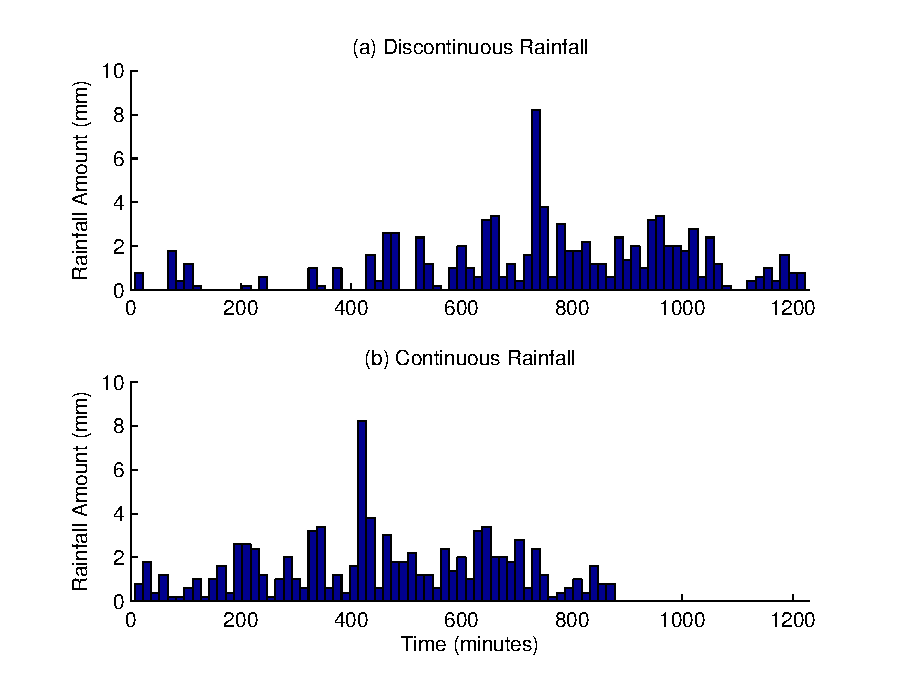
\includegraphics[width=1.0\textwidth]
{./img/rainfall_discont_cont_input}
  \caption[15-min rainfall data used for the investigations of effects of
continuous and discontinuous rainfall on soil erosion.]{15-min rainfall data
used for the investigations of effects of continuous and discontinuous rainfall
on soil erosion. (a) original 11 October 2000 event ;(b) modified 11 October
2000 event after removing WSGs}
  \label{fig:rainfall_discont_cont}
\end{figure}

A separate set of continuous and discontinuous rainfall data were prepared for
RillGrow simulations. Because RillGrow simulates runoff and soil loss in great
detail temporally and spatially, a rainfall event with a relatively short
duration---to reduce computational time---and a number of high intensity peaks
with a constant intensity were intentionally prepared (Figure
\ref{fig:rg2_input_continuous}). For this designed storm, constant intensity was
used because it made the shape of the storm simple. Also, it minimises any
unforeseen modelling interference from the changes of WSIV.
%For WEPP and EUROSEM simulations, constant intensity is not used because actual
%rainfall event is used.

\begin{figure}[tbp]
  \centering
    \subfloat[Continuous]{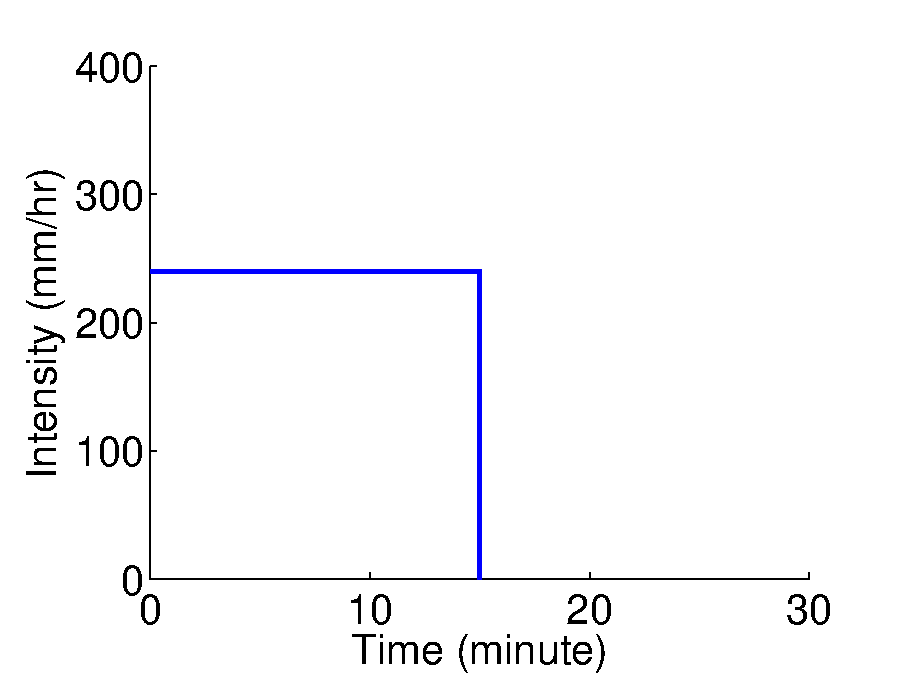
\includegraphics[width=0.5\textwidth]
{./img/rg2_input_continuous}}
    \subfloat[Discontinuous]{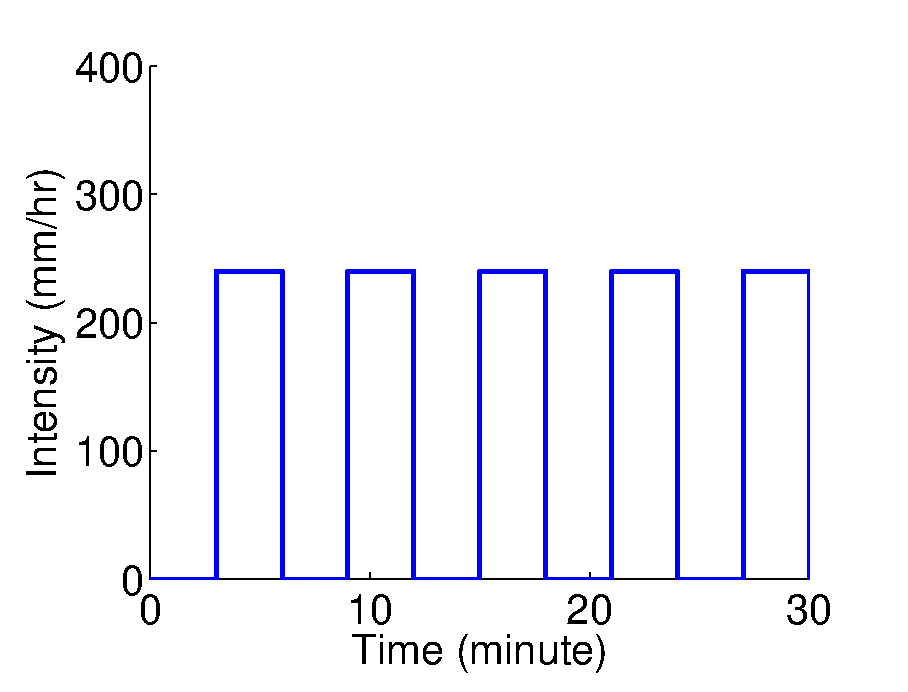
\includegraphics[width=0.5\textwidth]
{./img/rg2_input_discontinuous}}
  \caption{Continuous and Discontinuous rainfall for RillGrow simulations. Both
storms have the same total rainfall amount of 65.5 mm. Rainfall durations for
continuous (a) and discontinuous (b) rainfall are 15 minutes and 30 minutes,
respectively.}
  \label{fig:rg2_input_continuous}
\end{figure}

Simulated runoff and soil loss rates by WEPP, EUROSEM and RillGrow using
the prepared rainfall data are presented in the next section.

\section{Simulation Results}
\label{sec:InterStormGapsSimulatedResults}

\paragraph{WEPP simulation result} WEPP-estimated runoff amounts for continuous
and discontinuous rainfalls are shown in Table
\ref{tab:EstimatedRunoffForEachHillslope}. WEPP generated less runoff with
discontinuous rainfall than with continuous rainfall. WEPP-estimated runoff
decreased 10 percent when estimated with a discontinuous rainfall than with a
continuous rainfall. However, for soil loss, WEPP estimated more soil loss with
discontinuous rainfall than with continuous rainfall. The soil loss estimated by
WEPP increased 4.6 percent with discontinuous storm in comparison to the soil
loss rate with continuous storm.

\begin{table}[hbtp]
  \figureversion{tabular}
  \centering
  \caption{WEPP-estimated runoff and soil loss with continuous and discontinuous
rainfall for each hillslope}
  \label{tab:EstimatedRunoffForEachHillslope}
    \begin{tabular}{lll}
      \toprule
      & Runoff (mm)& Soil loss (t/ha) \\
      \midrule
      Continuous & 38.1 & 47.4 \\
      Discontinuous & 34.3 ($-$10.0) & 49.6 ($+$4.6)\\
      \bottomrule
      \multicolumn{3}{l}{\footnotesize Figures in (\ ) are the \% changes from
the result with a continuous storm.}
    \end{tabular}
\end{table}

\paragraph{EUROSEM simulation result} EUROSEM-estimated runoff and soil loss
rates for continuous and discontinuous rainfall are shown in Table
\ref{tab:EUROSEMEstimatedSoilLossRatesForEachHillslope}. EUROSEM generated a
lesser amount of runoff with discontinuous rainfall than with continuous
rainfall. Also, less soil loss was estimated by EUROSEM with discontinuous
rainfall than with continuous rainfall. Runoff and soil loss rates estimated
by EUROSEM decreased 11.9 and 12.7 percent, respectively, with discontinuous
storm in comparison to those with a continuous storm.

\begin{table}[hbtp]
  \figureversion{tabular}
  \centering
  \caption{EUROSEM-estimated runoff and soil loss with continuous and
discontinuous rainfall for each hillslope}
  \label{tab:EUROSEMEstimatedSoilLossRatesForEachHillslope}
    \begin{tabular}{lll}
      \toprule
                & Runoff (mm) & Soil loss (t/ha) \\
      \midrule
      Continuous & 28.7 & 11.0 \\
      Discontinuous & 25.3 ($-$11.9)& 9.6 ($-$12.7)\\
      \bottomrule
      \multicolumn{3}{l}{\footnotesize Figures in (\ ) are the \% changes from
the result with a continuous storm.}
    \end{tabular}
\end{table}

\paragraph{RillGrow simulation result} RillGrow-estimated soil loss rates for
continuous and discontinuous rainfall are shown in Table
\ref{tab:RillGrowRunoffAndSoilLossWithContAndDiscontRainfall}. RillGrow
generated slightly more runoff with discontinuous rainfall than that with
continuous rainfall. With discontinuous rainfall, runoff increased 0.2 percent
in comparison to runoff estimated with continuous rainfall. The simulated runoff
amounts were in fact almost the same. This is because no infiltration was
considered during the simulation. Thus, every rain ran off the edge of the
simulated plot. The infiltration component of RillGrow2 was inactive. The
current version of RillGrow, which is version 6, has resolved the problem and
has a working infiltration component (personal communication with the developer,
D. Favis-Mortlock, on 31 January 2012).

Yet RillGrow estimated slightly less soil loss with discontinuous rainfall than
with continuous rainfall. The soil loss rate was decreased one percent with the
discontinuous storm in comparison to the soil loss rate with the continuous
storm.

Despite the changes in runoff and soil loss, magnitudes of the change
were much smaller than changes observed in the WEPP and EUROSEM results.

\begin{table}[htbp]
  \figureversion{tabular}
  \centering
  \caption{RillGrow-simulated runoff and soil loss with continuous and
discontinuous rainfall}
  \label{tab:RillGrowRunoffAndSoilLossWithContAndDiscontRainfall}
    \begin{tabular}{lll}
      \toprule
  & Totals lost from edges (litre$^\dagger$) & Soil loss (t/ha) \\
      \midrule
      Continuous & 471.5 & 91.2 \\
      Discontinuous & 472.4 ($+$0.2)& 90.3 ($-$1.0)\\
      \bottomrule
      \multicolumn{3}{p{11cm}}{\footnotesize $^\dagger$ Because of the model
output parameter, total volumes of runoff was presented in litre. Figures in (\
) are the \% changes from the result with a continuous storm.}
    \end{tabular}
\end{table}

\section{Discussion}
\label{sec:InterStormPeriodsWithinAStormDiscussion}

\paragraph{Breakpoint or CLIGEN data} Using breakpoint data for a erosion
simulation prevents the loss of WSG information from the original data.
Therefore, it is reasonable to choose breakpoint data over CLIGEN data for
studies similar to the current research which investigates effects of rainfall
intensity changes on soil erosion in great detail. However, using breakpoint
data for continuous long-term simulation, for example, is realistically almost
impractical since preparing such inputs for erosion modelling is a very labour
intensive and tedious task. Regardless to say that temporally high resolution
data may well not be always available for a long period too. Thus, for some
cases, CLIGEN data, which removes WSGs from original rainfall data, are
inevitably chosen for erosion modelling studies. This investigation showed the
effect of removing WSGs during rainfall duration on erosion simulations.

\paragraph{Effect of removing WSGs on EUROSEM results} By removing WSGs, we
are unintentionally creating a rainfall event with higher average intensity than
the original average intensity as total storm duration becomes shortened. This
means that, first of all, the time given for the erosion simulation is decreased
so that smaller values of time-related parameters such as runoff duration are
used for other relevant process calculations. This will have an effect on, for
example, the time allowed for runoff initiation and development. Secondly, the
increased average intensity may increase on the erosional power of rain
storm. Thus, amounts of soil detachment and soil particles carried away by
surface flow could be increased. Depending on the dominant process, runoff and
soil loss could increase or decrease together.

Removing WSGs during a storm duration may result in, for example, increased
runoff and soil loss rates in comparison to those simulated with the original
rainfall because of increased erosive power of storm being more dominant than
the time reduced. This seemingly was the case for EUROSEM simulations (Table
\ref{tab:EUROSEMEstimatedSoilLossRatesForEachHillslope}).

EUROSEM showed significant impacts of WSGs on estimated runoff and soil loss. By
maintaining WSGs, runoff was simulated with almost 12\% smaller amount than by
removing WSGs. This reduction in runoff was corresponded with decreased soil
loss which was almost 13\% smaller than that of continuous storm. These results
imply that if runoff and soil loss are estimated by EUROSEM, the result could
vary over 10\% depending the existence of WSGs in breakpoint data. This figure,
of course, may well be specific to the storm that have been used here. In order
to find a more general magnitude of the impact, a further investigation may be
needed. Also, the relationship between magnitudes of changes and proportions of
WSGs in storms may need to be investigated. Nevertheless, even without any
further test, it is clear that WSGs do have impacts on EUROSEM-estimated runoff
and soil loss.
WEPP and RillGrow showed rather different results from the EUROSEM results,
however.

\paragraph{RillGrow without infiltration component} First of all, simulation
results from RillGrow runs showed very small differences between continuous and
discontinuous rainfall. In fact, the differences in runoff and soil loss between
two rainfalls were almost negligible. This, as mentioned previously, could have
been the result of the infiltration component not having been activated in
RillGrow. Thus, infiltration was not considered for the RillGrow simulations.

In comparison to RillGrow, however, the other two models, which have working
infiltration components, showed some degrees of changes in runoff and soil loss.
This implies that infiltration component plays an important role in making the
differences in the simulated runoff and soil loss rates. Thus, without the
working infiltration component, RillGrow2---the version of RillGrow that was
used in this investigation---was assumed to be not sensitive to WSGs.

The more improved version of RillGrow, which is in version 6, has functioning
infiltration component (personal communication with D. Favis-Mortlock in
December 2011).

\paragraph{Modification of original breakpoint data by WEPP}
\label{sec:WEPPModificationofBP} WEPP estimated more
soil loss with discontinuous rainfall than with continuous rainfall even though
runoff was decreased when simulated with discontinuous rainfall. This was
unexpected. If average rainfall intensity of a rainfall storm is
increased keeping the amount unchanged, the increased average intensity is
expected to produce more runoff and, in turn, more soil loss than low average
intensity. However, the opposite results were observed from the WEPP simulation
result.

By examining WEPP outputs thoroughly---including the WEPP outputs from
the previous chapter, Chapter \ref{sec:EFFECTSOFTEMPORALSCALESOFSTROMDATA}, it
was found that WEPP actually misinterpreted the intensity of the original
breakpoint data, and modified the original intensity
information before using them for estimating runoff and soil loss.

WEPP reconstructed a ``new'' rainfall storm based on the original breakpoint
data when the temporal resolution of rainfall data shorter than an hour were used.
This ``WEPP-modified'' rainfall storm had the same accumulated rainfall
amounts and the number of breakpoints from the original data, but the time
increments for each data point were changed. By changing the original time
increments, WEPP, in effect, changed the original rainfall intensity
information. The differences between the original breakpoint data and the
``WEPP-modified'' breakpoint data are illustrated in Figure
\ref{fig:intensity_discontinuous_and_continuous}. WEPP decreased intensity peaks
of continuous rainfall while it increased intensity peaks of continuous rainfall
as seen in Figure \ref{fig:intensity_discontinuous_and_continuous}.

\begin{figure}[htbp]
  \centering
    \subfloat[Continuous]{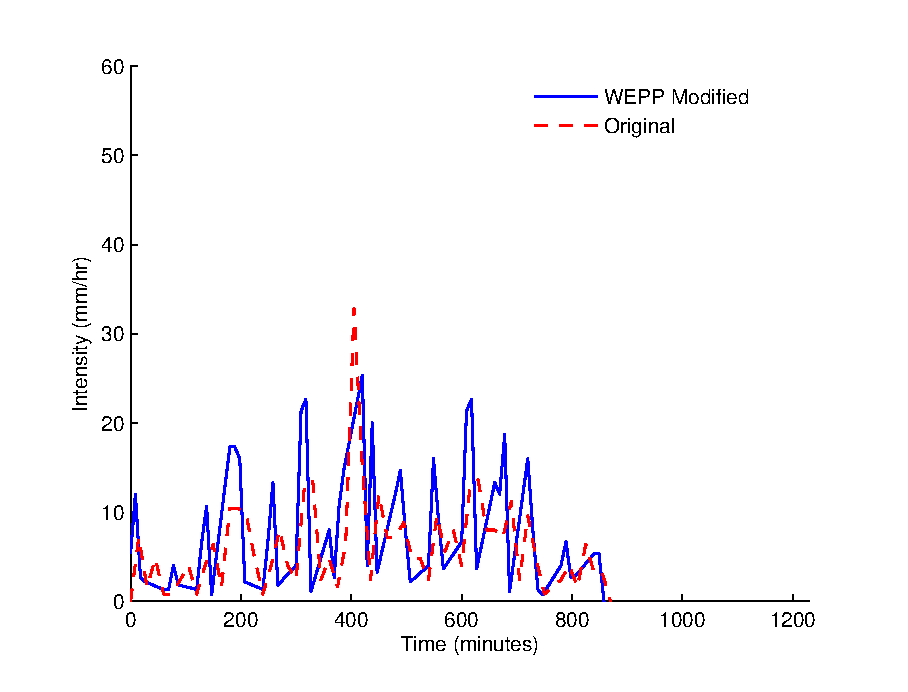
\includegraphics[width=0.5\textwidth]
{./img/intensity_continuous} \label{fig:intensity_continuous}}
    \subfloat[Discontinuous]{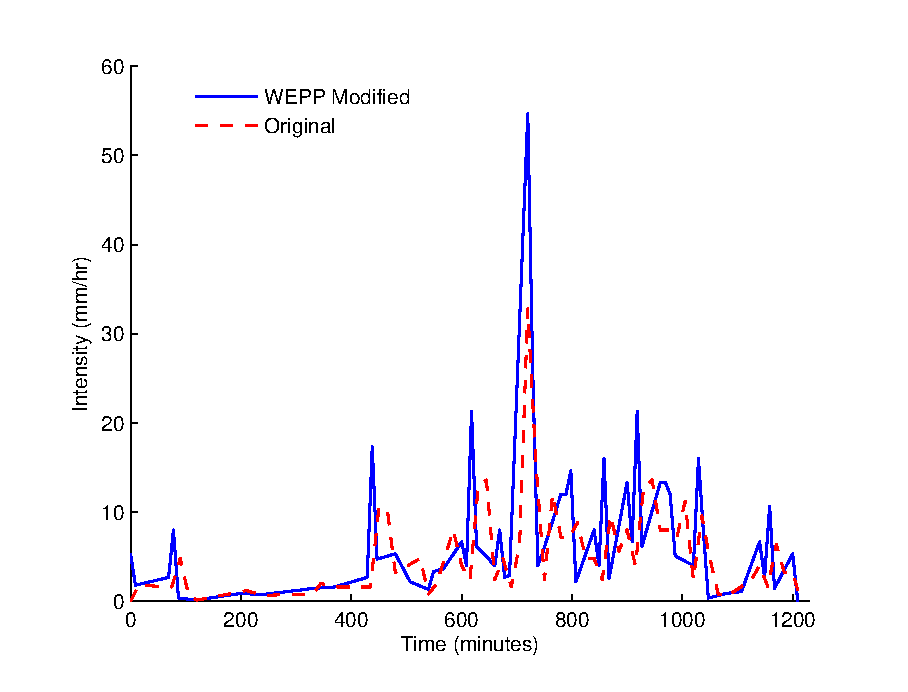
\includegraphics[width=0.5\textwidth]
{./img/intensity_discontinuous} \label{fig:intensity_discontinuous}}
  \caption{Original rainfall intensity and WEPP-modified rainfall intensity for
discontinuous and continuous rainfall.}
  \label{fig:intensity_discontinuous_and_continuous}
\end{figure}

The peak intensity of continuous rainfall was decreased from 32.8 mm/hr to 25.3
mm/hr (Table \ref{tab:summaryofweppchangedstormdetails}). This is about a 23\%
decrease in the peak intensity. The rainfall amount and total duration of
continuous rainfall were kept almost the same so that the average rainfall
intensity for the original data and WEPP-modified data were almost the same
(Table \ref{tab:summaryofweppchangedstormdetails}).
Also, the peak intensity of discontinuous rainfall was increased from 32.8 mm/hr
to 54.7 mm/hr (Table \ref{tab:summaryofweppchangedstormdetails}). The peak
intensity was increased about 67\%. Since the rainfall amount and total duration
of discontinuous rainfall were kept almost the same too, the average rainfall
intensity for the original data and WEPP modified data were almost the same.
These details are summarised in Table
\ref{tab:summaryofweppchangedstormdetails}.

\begin{table}[htbp]
  \figureversion{tabular}
  %\footnotesize
  \caption{Detailed summary of original and wepp-interpreted storm intensity
(mm/hr)}
\begin{tabular}{lrcrc}
  \toprule
 & \multicolumn{2}{c}{Continuous} & \multicolumn{2}{c}{Discontinuous} \\
  \cmidrule(r){2-3} \cmidrule(l){4-5}
 & Peak & Average & Peak & Average \\ \midrule
Original & 32.8 & 6.2  & 32.8 & 4.4 \\
Wepp-interpreted & 25.3 & 6.3 &  54.7 & 4.5 \\
Change (\%) & -22.9 &  & +66.8 &  \\
  \bottomrule
\multicolumn{5}{p{8cm}}{+/- denotes increase or decrease}
\end{tabular}
\label{tab:summaryofweppchangedstormdetails}
\end{table}

This finding poses a serious problem and, as far as only WEPP (with breakpoint
data) is concerned, has a substantial impact on our ability to investigate
impacts of rainfall intensity changes not only in the future but also in the
present. Without ability to process original intensity information, it is very
likely to end up with invalid results similar to the WEPP simulation result
shown in this chapter (see Table \ref{tab:EstimatedRunoffForEachHillslope}).

\section{Conclusion}
\label{sec:InterStormPeriodsWithinAStormConclusion}

Within-Storm Gaps (WSGs) have impacts on runoff and soil erosion simulated by
WEPP and EUROSEM except RillGrow. RillGrow showed almost no changes in
runoff and soil erosion simulation results because of the lack of functioning
infiltration component. Although it was not evident whether WSGs had positive
or negative effects on runoff and soil erosion estimations, removing WSGs from
original rainfall data affected the model simulation results. Thus, it is not
recommended to remove WSGs from the original rainfall data in order to
maintain the original rainfall intensity information. It is a best practice to
use rainfall data which have all necessary information for modelling.

Analyses of outputs from WEPP simulations revealed a new problem. WEPP modified
original rainfall intensity information and simulated erroneous results
(Table \ref{tab:EstimatedRunoffForEachHillslope}.  This is because that WEPP
constructs a ``WEPP-modified'' rainfall data based on original rainfall data
when breakpoint data with a temporal resolution shorter than 60-min temporal
resolution is
used for WEPP simulations. Particularly, peak rainfall intensity and the shapes
of rainfall storm are altered. This clearly is a major problem for current
research and for our ability to predict erosion. This is also a major model
fault for WEPP. This means that, even if 15-min breakpoint rainfall data---as
suggested in the previous chapter---are used for WEPP simulations, rainfall
data, which WEPP actually uses for the simulation, have different rainfall
intensity from the original data. This then leads to the estimation of
unrealistic soil erosion.



%\nolinenumbers

%but how much different? no can say about real world, but certainly
%important when models are used. this means it is important to know how much
%``gaps'' in the storm in order to predict future soil erosion, particularly
%in relation to rainfall intensity changes.
